\documentclass{llncs}
%
\usepackage{amsfonts}
\usepackage{amstext}
\usepackage{amsmath}
\usepackage{booktabs}
\usepackage{enumitem}
\usepackage{multirow}
\usepackage{graphicx}
\usepackage[center]{subfigure}
\usepackage{amssymb}
\usepackage{graphicx,amsmath} % Add all your packages here
\usepackage{subfigure}
\usepackage{algorithm}
\usepackage{algorithmic}
\renewcommand{\algorithmicrequire}{ \textbf{Input:}}
\renewcommand{\algorithmicensure}{ \textbf{Output:}}
\usepackage{url}
\usepackage{cite}
\usepackage{color}
%
\usepackage{CJK}

\begin{document}
\begin{CJK}{UTF8}{song}
\title{基于TSDF和Octrees的三维立体重建技术}
\author{刘畅}
\institute{School of Computer Science and Engineering, Beihang University, Beijing, China\\}
\maketitle

\begin{abstract}
本篇文献综述所讲述的主要内容是基于深度传感器,利用TSDF和Octrees等表面生成算法,对不同的相机移动路径计算方法,以及模型生成方法进行了介绍,比较各个方法的特点和优劣。同时,本文还对三维重建中常常出现的空洞修补工作进行了简单的介绍。最后,本篇文献综述对三维立体重建技术的难点进行了总结,并指出对立体重建未来的发展方向。
\keywords{三维立体重建技术, TSDF, Octree}
\end{abstract}

\section{Introduction}

计算机视觉是一门研究如何通过视觉传感器捕捉到的信息,对物体进行识别、分析的学科,而三维立体重建技术正是其子领域。现如今,三维立体重建技术被广泛应用于文物保护、游戏开发、医学研究、地图绘制等领域,例如对受灾地区进行三维重建以辅助救援\cite{DBLP:journals/mta/VerykokouIADA18},通过将传感器安装到机械臂上进行三维地图构建\cite{DBLP:journals/access/BanerjeeYA18},以及机器人自主控制\cite{DBLP:journals/jfr/LinGQGLWYS18,DBLP:conf/iros/WagnerFB14}等等。目前\cite{DBLP:journals/ral/FaulhammerABZFH17}提出了一种基于meta-room\cite{DBLP:conf/iros/AmbrusBFJ14}的机器人导航系统,但是这种系统需要进行一定量的重计算以及检查工作,而\cite{DBLP:conf/icra/FehrFDSGSC17}对此进行了改进。

三维重建的主要目的是根据传感器对某一物体或场景捕获到的若干图像或一段视频,将物体或场景通过一系列技术手段还原成三维立体模型。模型的重建主要依赖于深度相机,这种相机可以同时获取RGB图像和深度图像,前者记录被拍摄位置的颜色、亮度、饱和度等信息,后者通过某处灰度值大小反映出对应位置与相机间的距离,以此可以得到被拍摄场景的单方向模型。

目前,三维立体重建技术的主要难点是对相机移动的路径进行估算,以确定相邻两幅图形间的位置关系,以及图像的去燥、模型空洞的补全等等。这篇论文主要针对这些难点,论述近年来相关重建方法的种类以及改进方法。

\section{三维空间还原}

将深度照相机所获取的RGB图像与深度图像相结合,可以重建出每一个像素点在三维空间中的位置。设图像上某像素点$(p_x,P-y)$,通过深度图像$I_d$可以获得该像素点的深度值

\begin{equation}
\label{xy2z}
	z = I_d(p_x,p_y)
\end{equation}

根据公式\ref{xy2z}得到的结果,利用图像中心的坐标$(c_x,c_y)$和相机镜头到图片平面的距离$f$,可以通过函数$\rho$得到像素点$(p_x,P_y)$对应的三维坐标

\begin{equation}
\label{get3dpoint}
	\rho(p_x,p_y,z) = (\frac{p_x-c_x}{f}z,\frac{p_y-c_y}{f}z,z)
\end{equation}

我们将每组图像中每个像素还原得到的三维点的集合称为“点云(Point Cloud)”。

\cite{DBLP:conf/aaai/LinKL18}提出了一种高效生成点云的方法,该方法提出了pseudo-renderer模型,使用二维卷积运算通过多视角对三维模型进行预测,并且利用二维投影优化进行几何推理,最终的生成结果具有良好的形状相似性和较高的预测密度。


\section{主要的表面生成方法}

点云所表现出的结果是离散的,于是接下来的工作是,根据每一组图像得到的点云生成连续的物体表面,并将所有图像所生成的结果合并,得到完整的三维模型。目前两种方法被应用得较为广泛,分别是截断有向距离函数(Truncated Signed Distance Function, TSDF)和八叉树(Octrees)。

	\subsection{截断有向距离函数(truncated signed distance function, TSDF)}

早期曾提出一种利用截断有向距离函数生成模型表面的做法\cite{DBLP:conf/siggraph/CurlessL96},其主要原理是对于单幅深度图像,三维空间中某一点$p$可用函数$d(p)$表示到表面的距离:当$d(p)>0$的时候,认为$p$在表面后方(远离相机位置);当$d(p)<0$的时候,认为$p$在表面前方(靠近相机位置);而当$d(p)=0$的时候,即可认为$p$正好处于表面上。

对于由深度图像像素还原得到的点$P_0$,可以认为$d(p_0)$接近于0。为了提高结果的准确性,这里对于表面附近不同图像、不同位置的点,分别给予了不同的权重w,利用各个点的权重$d(p)$和距离函数$w(p)$,根据公式\ref{D_cal}和\ref{W_cal}对空间中划分的离散体素网格进行权重$W$和距离$D$的更新,最终得到一个较为准确的$D(p)=0$的表面。

\begin{equation}
\label{D_cal}
	D(p) = \frac{\sum w_i(p)d_i(p)}{\sum w_i(p)}
\end{equation}

\begin{equation}
\label{W_cal}
	W(p) = \sum w_i(p)
\end{equation}

TSDF往往能得到较为准确的重建结果,如\cite{DBLP:conf/cvpr/FioraioTFSI15,DBLP:conf/icra/ForsterPS14},但是当这种方法被应用于较大模型重建的时候,由于信息量的增多,会导致内存消耗很大。

目前TSDF作为主流的三维立体重建方法之一,依然被广泛使用,如\cite{DBLP:journals/corr/abs-1710-07242}基于TSDF提出了一种限制点云扩增的方法,用于生成稳定的密集三维点云系统。

%在此方法的基础上,\cite{DBLP:conf/rss/KlingensmithDSX15}和\cite{Whelan2013Deformation}


%采用了一种截断有向距离函数(Signed Distance Function, TSDF)

%TSDF是主要应用在三维重建技术中的一种确定模型表面的方法,是对Signed Distance Function(SDF)的一种改进。

	\subsection{八叉树}
八叉树是一种每个父节点拥有八个子节点的树\cite{Wurm2010OctoMap},树中的每个结点都可用来表示空间中的一个立方体,每个子节点所代表的立方体都是父节点立方体的$\frac{1}{8}$,如图\ref{Octree}所示。用八叉树表示空间的方式的优点是可以动态地调整空间的精细度,当需要对物体进行更高精度的描绘时,可以增加八叉树的深度,细化空间单位;当需要节省内存的时候,可以使用较大的立方体表示空间,提高效率。

\begin{figure}
\centering
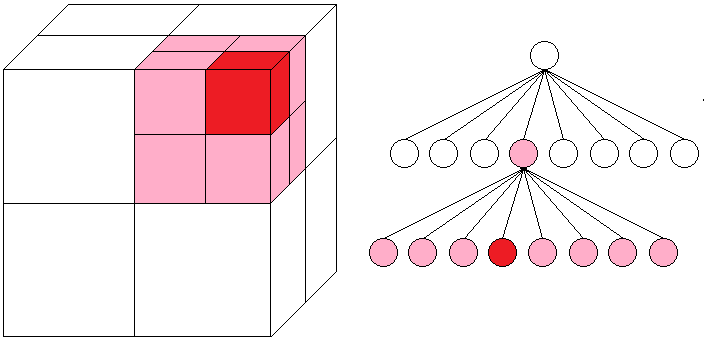
\includegraphics[width=0.8\textwidth]{picts/octree.png}
\caption{递归分割空间的八叉树}
\label{Octree}
\end{figure}

利用八叉树绘制表面的方式是对立方体进行标记——如果该立方体占有的空间中包含了表面上的点,那么就将该立方体细分并标记为“占有”,否则就将其标记为“空闲”。这种方式更加高效,可以处理规模较大的模型。目前,八叉树不仅被应用于三维立体重建技术\cite{DBLP:conf/icra/SenguptaS15},还被应用于多层寻路\cite{DBLP:journals/cgf/JiaZYP18}等领域,具有广泛的应用价值。


\section{相机追踪与模型生成}

所谓相机追踪,是指在三维空间还原中,每幅图像生成的点云所属的坐标系是以相机所处位置为基准确定的,但相机在拍摄的过程中是保持移动的,因此不同点云采用的是不同的坐标系。为了将不同点云进行融合,必须要统一坐标系,因此必须确定相机所处的位置。

拍摄相邻两幅图像时相机的位置变化可以用旋转量$R$和位移量$t$来表示,目前有很多方法可以实现对$R$和$t$的估算。在确定了相机的位置之后,就可以综合之前生成表面的方法,对被拍摄物体或场景进行模型的生成。

	\subsection{迭代最近点(Iterated Closest Point, ICP)}

迭代最近点的主要工作是对两组相邻点云进行点与点之间的配对,然后计算出旋转量$R$和位移量$t$,将其中一组点云转化为另一组点云,并使得花费$E$最小\cite{DBLP:journals/pami/BeslM92}。其中,$E$的计算方式是转换后两组点云中对应点的位置差异之和。

我们假设原点云为$x_1,x_2,...,x_n$,目标点云为$y_1,y_2,...,y_n$,则需要最小化的花费可表示为

\begin{equation}
\label{cloudpoint_min}
	E(R,t) = \sum_{i=1}^n||Rx_i+t-y_i||^p
\end{equation}

对于已经确定配对关系$(x_i,x_i)$的两组点云,通过调整$R$和$t$的值,使得公式\ref{cloudpoint_min}的值降到最低。对于指数$p$的取值,通常为$p=1$或$p=2$。

然而,找到最符合实际变化的旋转量$R$和位移量$t$的前提是配对$(x_i,x_i)$的正确。为了提高配对的准确性,这里采用迭代的方式不断优化点云间的配对关系,如图\ref{ICPfig}所示。主要步骤如下:

\begin{enumerate}
\item{决定初始的配对关系}
\item{利用公式\ref{cloudpoint_min}找到合适的旋转量$R$和位移量$t$}
\item{采用此种转换方式对原点云$x$进行转换,得到转换后的原点云}
\item{重复步骤1\~{}3直到$E(R,t)$的值不发生明显变化}
\end{enumerate}

\begin{figure}[htbp]
\centering
\subfigure[第一次配对]{
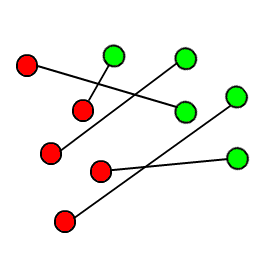
\includegraphics[width=0.4\textwidth]{picts/first_pair.png}} \\
\subfigure[第二次配对]{
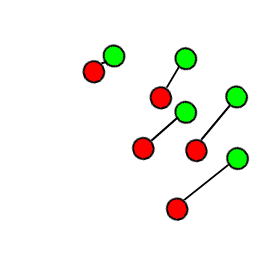
\includegraphics[width=0.4\textwidth]{picts/sec_pair.png}}
\subfigure[最终结果]{
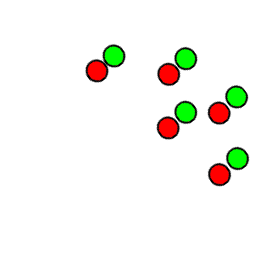
\includegraphics[width=0.4\textwidth]{picts/third_pair.png}}
\caption{使用ICP方法进行点云间点匹配}
\label{ICPfig}
\end{figure}

当原点云与目标点云差异较小的时候,这种方法有较大概率找到全局最优解;但是当原点云和目标点云差异较大的时候,往往会使结果陷入局部最优解。

在此基础上,一种采用结合了法线的改进方法被提出\cite{Chen1992Object},这种方法以最小化原点云中$x_i$的法线$n_i$与$x_i$和$y_i$间连线$L(x_i,y_i)$投影之和的方式代替了原来的单纯地最小化两点间距离之和的方法,即

\begin{equation}
E'(R,t) = |(Rx_i+t-y_i)^Tn_i|^p
\end{equation}

ICP方法具有它的局限性,对于点云上所有点位于同一平面的情况,用ICP方法求解得到旋转量$R$和位移量$t$并不唯一。

2011年,微软提出了一种经典的重建模型方法——KinectFusion。KinectFusion\cite{DBLP:conf/ismar/NewcombeIHMKDKSHF11}的伟大之处在于它实现了通过传感器实时生成3D模型的功能,具有极高的实用性。它使用ICP方法进行相机移动路径的追踪,使用TSDF方法有效地对中等大小的模型进行表面构造,并使用\cite{DBLP:conf/siggraph/CurlessL96}的方法建立3D模型。有很多类似的方法曾被提出\cite{DBLP:conf/cimaging/KubackiBBD12,DBLP:conf/eccv/RenR12},但是前者使用的测试数据是人造的,且缺乏合理的评估方法;后者的SDF函数是已知的,且缺乏实时性。KinectFusion可以进行可靠的即时渲染,并同时生成两组点云——一组是根据当前深度图像生成的,另一组是之前所有深度图像生成点云的合并,当所有图像都被处理完毕后,后者即为全局的点云结果。

此后,微软研发出了一种全新的、用于读取RGB信息和深度信息的驱动Kinect V1,在此之上诞生很多经典的三维重建方法,如一种高效的融合深度图像冗余信息的技术\cite{DBLP:conf/scia/KyostilaCKH13}。随后微软开发了Kinect V2驱动,\cite{DBLP:conf/scia/YlimakiKH17}基于此驱动提高了此前方法的鲁棒性,减小了离群点的数量,但是使用这种方法生成的表面有明显的模糊和粗糙效果。这种缺点在\cite{DBLP:journals/corr/abs-1804-08912}中被改进,且依然具有较高的可靠性。

为了提高效率,\cite{DBLP:journals/tog/NiessnerZIS13}提出了spatial hashing方法,并开发了一个重建大规模模型的实时系统,这种方法基于体素的哈希映射,有效提高了运行效率并降低了内存的消耗,并被应用于移动设备的CPU计算\cite{DBLP:conf/rss/KlingensmithDSX15}。




	\subsection{图像一致性比对}

对于每组图像中的深度图像$I^n_d$和RGB图像$I^n_c$,其下一组图像中深度图像和RGB图像分别为$I^{n+1}_d$和$I^{n+1}_c$。图像一致性比对方法的主要工作是先利用公式\ref{get3dpoint},根据$(I^n_d,I^n_c)$还原出点云$P^n$,之后选取适当的旋转量$R$和位移量$t$对$P^n$进行变换,并映射到平面$\pi$上\cite{DBLP:conf/iccvw/SteinbruckerSC11}。在理想情况下,映射到平面$\pi$上的RGB图像应当与$I^{n+1}_c$完全一致。但由于误差的存在以及$(R,t)$的选取,两图像间应当存在差异,这时需要动态调整$(R,t)$的选值,尽可能减少$I^{n+1}_c$上各点$(i,j)$和平面上对应点$\pi(p)$的色度差异,其差异可用公式\ref{IBMdif}表示:

\begin{equation}
\label{IBMdif}
E(R,t) = \sum^m_{i=1}\sum^n_{j=1}||I^{n+1}_c(i,j)-I^n_c(\pi(R\rho(i,j,z_{ij})+t))||^2
\end{equation}

其中,$z_{ij}$是根据公式\ref{xy2z}得到的图像$I^n_d$中点$(i,j)$的深度值,$m$和$n$表示图像的高度和宽度。除了色度差异外,这种方法也可通过比较深度差异进行$(R,t)$的计算\cite{Kerl2013Large}。和ICP不同的是,ICP是对两组图像生成的点云进行比较,而图像一致性比对是对二维图像进行比较,其优点在于有效利用了图像的色度信息,并且不需要对两组点云中的点进行匹配。

有很多基于图像一致性比对的模型生成技术\cite{6631104,DBLP:conf/iros/KerlSC13},但是它们共性的缺点是生成的效果与实际误差较大,这是由于对相机移动路径的错误估计造成的。在图像一致性比对方法中,每一次计算出的旋转量和位移量具有一定误差,这种误差会随着图像组数的增多而累积,最终导致生成的模型与实际具有较大的偏差。目前,有很多减小误差的方法,例如loop-closure\cite{DBLP:conf/eccv/KahlerPM16,DBLP:journals/corr/abs-1708-00783}和bundle-adjustment\cite{DBLP:journals/ijcv/UrbanWLH17}。

	\subsection{图像关键点比对}

图像关键点比对方法是找出相邻两组图像之间一致的“关键点”,该方法使用了随机抽样一致算法(random sample consensus, RANSAC)计算相机位置的变化,并将之存储在表中\cite{DBLP:conf/icra/EndresHESCB12},这样做的目的是对相机移动路径的计算精度进行优化,防止误差的累积。当所有数据被收集完毕之后,\cite{DBLP:conf/icra/EndresHESCB12}使用了八叉树进行表面的生成,并使用$G^2o$方法进行优化\cite{DBLP:conf/icra/KummerleGSKB11}。

由于这种方式是通过提取图像中的关键点进行计算而非对整个图像进行比较,因此处理效率相比于ICP更高。但是这种方法的弊端是不支持实时建模,必须要等到所有数据都被存储之后才可以生成模型。

	\subsection{ICP和图像一致性比对的结合方法}

这种方法结合了基于ICP的KinectFusion方法和图像一致性比对方法,用于对相机的移动轨迹进行计算,例如Kintinuous\cite{DBLP:conf/icra/WhelanJKLM13}和Elasticfusion\cite{DBLP:conf/rss/WhelanLSGD15}。这是一种实时计算的方法,可以用于较大尺寸的模型重建。为了实现这一点,这种方法可以有效地减小误差的累积,提高重建的精密度。

Kintinuous\cite{DBLP:conf/icra/WhelanJKLM13}提出了一种减小内存开销的算法,通过对空间划分网格实现空间的单位化,当相机达到网格的边缘后,已经经过的部分空间就会在内存中被释放,同时为下一块网格分配新的内存空间,限制了内存的使用。

Elasticfusion使用了surfels方法\cite{DBLP:conf/siggraph/PfisterZBG00}生成表面,由于surfels方法对表面信息的记录更为全面,因此当出现误差的是时候,可以很方便地进行检查或重计算,保证了算法的可靠性,因此结果较为理想。

\section{空洞的检测}

三维立体建模中常见的空洞包括三种:扁平空洞、岛状空洞以及缝隙空洞\cite{DBLP:journals/vc/GuoXW18},如图\ref{holeType}所示。

\begin{figure}[htbp]
\centering
\subfigure[扁平空洞]{
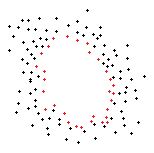
\includegraphics[width=0.4\textwidth]{picts/flat.png}} \\
\subfigure[岛状空洞]{
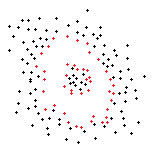
\includegraphics[width=0.4\textwidth]{picts/island.png}}
\subfigure[缝隙空洞]{
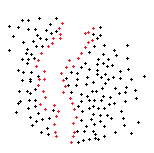
\includegraphics[width=0.4\textwidth]{picts/gap.png}}
\caption{在处理点云中常见的空洞类型}
\label{holeType}
\end{figure}

对于空洞的检测,可以将点云中的点分为边缘点和内陆点两种,而边缘点所围成的区域即为空洞。判断边缘点和内陆点的基本方法主要有angle criterion\cite{DBLP:journals/jwscg/BendelsSK06}half-disc criterion\cite{DBLP:journals/dm/WagnerW09},其它的还有一些基于这些方法的改进方法\cite{DBLP:conf/mm/ZhangW12}。除了需要检测空洞的存在,空洞的类型也需要进行判断,以决定空洞填补的策略。其中\cite{DBLP:conf/smi/WeberHH10}采用了尖锐特征检测的方法用于对较复杂的几何图形进行重建,而\cite{Tran2015Extraction}将杂乱的散点和基本的几何形状进行匹配,对空洞周围的点排列进行简化。


\section{总结}

本篇文献综述主要针对基于TSDF和Octrees等三维立体重建方法进行了介绍,这些方法都在其适合的领域内达到了较好的效果,如表1所示。同时,本文还对三维立体重建过程中的常见问题——空洞的处理进行了简单介绍。

\begin{table}
\label{sum}
\caption{一般建模方法的特征总结}
\centering
\begin{tabular}{cccc}
\toprule
\textbf{方法名}& \textbf{表面生成方法}& \textbf{适合大小}& \textbf{实时生成}\\
\midrule
KinectFusion& TSDF& 中等尺寸& √\\
图像关键点比对& Octrees& 皆可& ×\\
KinectFusion& TSDF& 较大尺寸& √\\
Elasticfusion& surfels& 较大尺寸& √\\
\bottomrule
\end{tabular}
\end{table}

由于深度相机全部根据RGB图像和深度图像对物体进行还原,无法对此外的信息进行获取,因此不同角度光照角度的变化、物体的运动等等都可能干扰到模型的生成。同时,在生成模型的过程中,暂时很难对由于噪声产生的空洞和模型本身自带的空洞进行区分,这可能会导致修补了不该修补的空洞,破坏了模型的结构。

未来,三维立体重建技术将重点投入在如何更佳高效、准确地重建模型,并对异常信息进行修正或屏蔽。同时,由于模型的生成高度依赖RGB图像和深度图像,因此提高图片精度可以有效应对更佳复杂的模型的重建。

\bibliographystyle{splncs03}
%\bibliographystyle{unsrt}
\bibliography{reference}
\end{CJK}
\end{document} 
